\chapter{Prototype development}
\label{chap: Chapter 6}

Chapter \ref{chap: Chapter 5} introduced the conceptual model. This chapter will discuss everything that is needed to develop the prototype and performing the experiments. The prototype essentially provides an implementation of the conceptual model defined in Chapter \ref{chap: Chapter 5}.

\begin{figure}[h!]
\centering
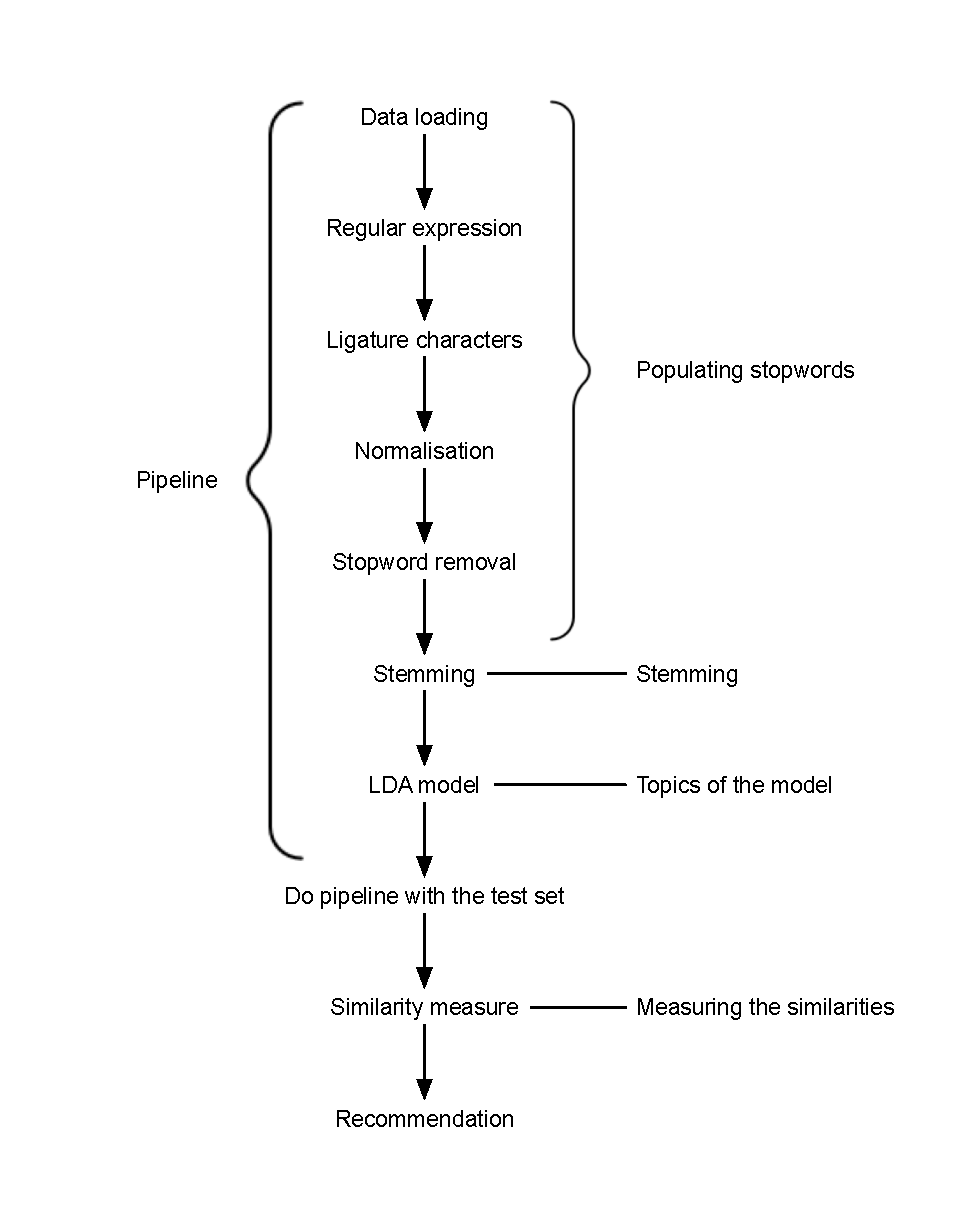
\includegraphics[width=12cm]{./figures/flowresearch12.eps}
\caption{High level overview of the prototype}
\label{fig:prototype}
\end{figure}

The rest of the chapter will look at each element in the pipeline, as depicted in Figure \ref{fig:prototype}, especially with the focus on the refinements that were applied. Figure \ref{fig:prototype} illustrates the steps that were followed in the creation of the prototype. Furthermore, Figure \ref{fig:prototype} shows mappings from the prototype development and refinement to the various parts which were created in the conceptual model chapter, in Chapter \ref{chap: Chapter 5}. In addition, the parts that were intentionally neglected will also be discussed. This chapter will start with a overview of the development of the prototype.

\section{Prototype overview}

The prototype can be split up into four parts at a system level view: (1) identification and removal of the stopwords, (2) stemming the text, (3) topics of the model, and (4) similarity measurement between the test and training set. Although the identification and removal of stopwords and stemming can be grouped under pre-processing, it is important to note that each has an important role in the development of the prototype. Each part plays a critical role in how usable the text is for further topics modeling. Stopword identification and removal is a process that is applied the same in the learning phase and testing phase of the prototype, the same goes for stemming.

As mentioned in section \ref{ssec:model}, it is utmost important to develop a prototype to validate a model. There will always be lesson to be learned, which will be discussed in chapter \ref{chap: Chapter 7}.

The prototype was developed to achieve the following goals:

\begin{enumerate}
    \item To better understand the problem domain, the research problem, and the solution.
    \item To show that the natural language processing and topic modeling approach is feasible.
    \item To be used in recommending research papers and to see the relevance of those recommendations made from the prototype.
\end{enumerate}

The prototype has undergone three iterations, which have supported the goals stated above. The first iteration tied in with the first goal, to better understand the domain and to explore a possible solution. The first iteration provided insight by exploring how recommender systems work and the techniques employed to achieve the desired goal. The second iteration focused more on the initial pre-processing phase of the prototype along with the topic modeling algorithm, latent dirichlet allocation (LDA), and what is to be learned from the development. The topics were later analysed to assess whether this approach will be sufficient. Lastly, the third iteration of the prototype was more polished and had refinement applied to it. The focus shifted slightly from NLP and topic modeling to better the quality of the recommendations made by the prototype. Throughout the third iteration, several parameters in the LDA algorithm were changed to better the recommendations. Unless specified otherwise, reference to the prototype will imply the usage of the third iteration of the prototype.

The researcher decided on Python as the base development environment. Python is a programming language that has gained its popularity in recent years for its modularity and effectiveness of handling data. Many developers have built various libraries in aiding the machine learning and information retrieval community with better system building.

More specifically, the researcher used Jupyter Notebook to build and test the prototype. Jupyter Notebook is a web application, which provides a Python development environment for users. Jupyter Notebook can be used in various ways: data cleaning, data transformation, statistical modelling, data visualisation and machine learning. It allows you to create and share documents that contain live coding, visualisations, and text, thus making it perfect for reproducability of the prototype and making the experimentation easier.
Every part of the prototype will now be discussed along with the various components related to each part.

Code snippets were used from:

https://github.com/JuandrevanHeerden/Juandre-M-Final

\section{Identification and removal of stopwords} \label{ssec:pre}

More frequently than not, looking for papers and analysing them is a daunting task for most researchers. The problem is that those papers found by researchers have too much noise to do the necessary, thus creating the need to clear all the unwanted noise from the text. One of the processes within pre-processing is called stopword removal.

Pre-processing contains many techniques to clear the text and make it ready for analysis. These techniques are primarily used in text mining pipelines to better the text input into Information retrieval systems. These techniques include tokenisation, stopword removal, and stemming and transforming the data into a vector space later in various text mining algorithms.

Before stopwords can be removed, they first need to be identified. Each document that needs to be pre-processed contains domain knowledge that is not shared across other domains. Specific domain knowledge needs to be identified first, and then certain words need to be applied to the stopword list. First the data needs to be extracted and analysed. In the next sub-section, we will discuss how the data was extracted. After that, we will discuss the steps taken to identify domain-specific words and add them to the stopword list.

\subsection{Extracting the data}

The data used in this study was obtained from the International Information Security South Africa Conference website. The articles were downloaded and documented in a per year fashion. The abstracts, along with the title of each article, were manually extracted into the form of ten csv files as seen in Figure \ref{\ref{fig:github}}. Each csv file had two columns named title and abstract. 

\begin{figure}[h!]
\centering
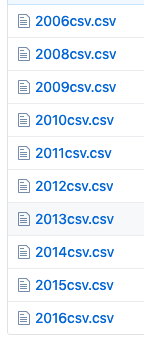
\includegraphics[width=2cm]{./figures/github.png}
\caption{Data on Github}
\label{fig:github}
\end{figure}

The collection of csv file were uploaded to github for documentation and reproducible purposes. A Python library called Pandas was used to handle the data, as seen in Figure \ref{lst:data}. Pandas is a well known library, which is primarily used to manipulate data.

\begin{lstlisting}[language=Python, label={lst:data}, caption=Importing data to the system]
# Import Dataset
df = pd.read_csv('https://raw.githubusercontent.com/brix-mix/Fake/master/2006csv.csv', usecols = ['abstracts','title'])
df1 = pd.read_csv('https://raw.githubusercontent.com/brix-mix/Fake/master/2008csv.csv', usecols = ['abstracts','title'])
frames = [df, df1]
df = pd.concat(frames, ignore_index=True)
df.head()
\end{lstlisting}

The dataset consists of 254 documents spread over 10 years. As shown in Figure 6.3, the largest document has 235 words, whereas the document with the least number of words has 10. The average number of words in the documents are 110. What this means is that there are about  20 per cent of the words that will actually have meaning. Usually, out of 100 words used in a piece of writing, 20 have meaning; the rest are filler words or stopwords.

\begin{figure}[h!]
\centering
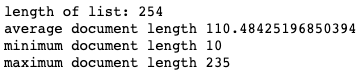
\includegraphics[width=6cm]{./figures/docstats.png}
\caption{Statistics of the documents}
\label{fig:data}
\end{figure}

It is best practice to remove all the stopwords and unwanted characters from your dataset. Junk in equals junk out. In order to achieve good results, a decision was made to clear the text of unwanted characters. The next sub-section includes further removal of unwanted text.

\subsection{Regular expressions}

Regular expressions can be seen as a sequence of characters that can be used to search for patterns, and those patterns are used to find and replace those characters. The nature of the domain of the document suggests that email addresses and other unconventional characters could be found in the text, therefore Figure \ref{lst:re} was used to remove these characters.

\begin{lstlisting}[language=Python, label={lst:re}, caption=Regular Expression]
text = re.sub("((\S+)?(http(s)?)(\S+))|((\S+)?(www)(\S+))|((\S+)?(\@)(\S+)?)", " ", text)
\end{lstlisting}

This code segment was only run once because all data were already in one big data frame. Looking at the raw text, the researcher found ligature characters, which also needed to be removed and replaced. In the next sub-section more details are discussed.

\subsection{Ligature Characters} \label{ssec:ligature}

In writing or typography, two or more characters can be merged into one to form; a glyph or single character called a ligature. Ligature characters were commonly used in \TeX{}. \TeX{} is a formatting system that was created and made famous in academia. The ease of executing specific typesetting tasks gave \TeX{} its popularity.

This research dataset contains older papers published from 2006 onwards, making it ligature prone. The two ligatures that were found in this research were; fi and fl. The main reason to replace these ligatures is to normalise the text, so that readers who do not change their font encodings will have no problem reading it. 
As seen in Listing \ref{lst:ligature}, the use of regular expressions was employed to find and replace the ligatures, fi and fl, respectively.

\begin{lstlisting}[language=Python, label={lst:ligature}, caption=Replacing Ligature Characters]
    # Remove fi and fl ligature characters
    text = re.sub("fi", "fi", text)
    text = re.sub("fi", "fl", text)
\end{lstlisting}

After removing the ligature characters, the normalised, tokenised text is ready for the stopwords to be removed.

\subsection{Stopword Removal}



A stopword can be defined as a word that is commonly used within a sentence. However, stopwords in this study are standard information security terms that need to be filtered out to enhance the quality of the topics. This was a delicate tweaking process. Only after the data were tokenised and viewed by the researcher a call was made to include several terms. The additional terms that was added was appended to the stopword list as seen in Listing \ref{lst:stopword}, the total number of stopwords totaled 282. After the filler words were excluded from the corpus, the next step in the pipeline is to stem the words.

\begin{lstlisting}[language=Python,label={lst:stopword}, caption=Stopwords code]
stop_words = stopwords.words('english')
stop_words.extend(['used','using','jam','found','plays','information','security','network', 'technology', 'bgp'])
\end{lstlisting}

\section{Stemming}

As mentioned in Chapter \ref{chap: Chapter 5}, Section \ref{ssec:stemming}, the Porter stemmer is used in the research \cite{porter1980algorithm}. The goal of a stemmer is to reduce the forms of a word to the common base word. Stemmers usually cut off the end part (affixes) to achieve above goal.
Stemmers are easy to implement and do not need time or resources to complete the task. This research looked at high performance, low time, or resources spent on normalisation of words. Stemming was selected to be used in this study based on its simplicity and the time it takes.
In Listing \ref{lst:stemming}, we display the code snippet showing how the stemmer was used.

\begin{lstlisting}[language=Python, label={lst:stemming}, caption=Stemming the corpus]
stemmer = PorterStemmer()
def stem_words(text):
    """
    Function to stem words, so plural and singular are treated the same
    """
    try:
        text = [stemmer.stem(word) for word in text]
        text = [word for word in text if len(word) > 1] #make sure we have no 1 letter words
    except IndexError: # catch the exception
        pass
    return text

\end{lstlisting}

In Listing \ref{lst:stemming}, the core code was to instantiate the Porter stemmer and feed the data through it. We also encountered some words like ’eod’, which  broke this and needed to insert a try catch, to make the code continue running.

\begin{table}[htbp]
\centering
\begin{tabular}{|l|l|}
\hline
\textbf{Word} & \textbf{Stemmed word} \\ \hline
informational & inform \\ \hline
translations & translat \\ \hline
evaluating & evalu \\ \hline
itemisation & item \\ \hline
awareness & awar \\ \hline
reference & refer \\ \hline
plotted & plot \\ \hline
\end{tabular}
\caption{Stemming words from the data}
\label{tab:stemming}
\end{table}


Some of the words that were found in the data along with their root forms can be viewed in Table \ref{tab:stemming}. The Porter stemmer takes the original word back to its root form.

In the next section, getting topics for the model will be discussed.

\section{Topics for the model}

This section will be a in-depth continuation of Chapter \ref{chap: Chapter 5}, Section \ref{ssec:topic}. The bag of words was the step taken between normalising the data and feeding it into a topic modeling algorithm. Later in this section, the topic modeling technique and its parameter refinement will be discussed.

\subsection{Bag of Words}

For the topic modeling technique to compute the latent topics, it needs to understand the document. Before the text gets to the topic modeling technique, the text is just tokenised and normalised, thus creating the need to represent the text in a manner that the topic modeling technique can interpret it. The most common technique in natural language processing and information retrieval is the bag of words (BoW) model.

The bag of words (BoW) model can be used to extract features from the text. A BoW model is a way to simplify the representation of words in a document. Note that it is called a ’bag of words’, the order of the words or sentence of the words does not bear merit. The BoW model is only interested in known words in the document, and the rest is discarded. \citeA{goldberg2017neural} mentions that documents are similar if they have similar content. The BoW model can be simple to use or rather complex in determining the vocabulary of known words and how to score the reoccurring words.

Determining the vocabulary will be shown below. Listed are snippets from a paper dealing with Phishing attacks occurring through email and social networking sites. Each sentence will be handled as a document. Ignoring case and punctuation, the sentences are:

\begin{itemize}
    \item Phishers continuously seek new methods... 
    \item Conducting phishing solely through email...
    \item Social network phishing and discusses...
\end{itemize}
After removing stopwords. The unique words here are:
\begin{enumerate}
    \item 'Phish'
    \item 'Method'
    \item 'Conduct'
    \item 'Email'
    \item 'Social'
    \item 'Network'
\end{enumerate}

This is a vocabulary of six words from a corpus of 15 words. Scoring the words can commence once the vocabulary has been selected. There are two scoring approaches one can follow. They are:

\begin{enumerate}
    \item Counting the number of times the word is used in the corpus.
    \item Frequencies can be calculated by how frequently each word is used out of all the other words.
\end{enumerate}

This research employed the first scoring approach by counting the words. A library called Gensim with a function of doc2bow was used to count the number of times the word occurs, converts the word to a word id and then returns the result as a sparse vector \cite{rehurek2010software}. Scoring the previous three documents against the vocabulary of six words will look as follows:

\begin{lstlisting}[language=Text, label={lst:scoring}, caption=Scoring the documents]
    Phishers continuously seek new methods = [1, 0, 0, 0, 0]
    Conducting phishing solely through email = [1, 1, 0, 0, 1]
    Social network phishing and discusses = [1, 1, 1, 0, 0]
\end{lstlisting}

Each sentence in Listing \ref{lst:scoring} was compared to the tokenised and normalised list. In conclusion, the BOW model disregards context, the meaning of the words, and lastly, the order in which the words appear. This gives the BOW model its strength because the more similar words are, the more similar documents are to each other. In the next subsection, we will discuss how the vector (BOW) is used in the topic modeling technique.

\subsection{Topic modeling parameters} \label{ssec:LDA}

In Chapter \ref{chap: Chapter 3}, this study discussed what latent dirichlet allocation is and how it works. In this section, we will discuss how the LDA algorithm parameters work, on a deeper level. It should be said that in latent dirichlet allocation the order of the words do not matter, because of the bag of words model used in the study.

The dataset consists of several documents, and a document is a distribution over topics. Each topic within the document is a distribution over words that is then added to a vocabulary. Latent dirichlet allocation is a probabilistic model that identifies hidden variables within text. To infer such variables using LDA, the algorithm has parameters that steer the inference process. These parameters include the number of topics, chunksize, corpus, minimum probability, id2word, alpha, and beta. The last two parameters, alpha and beta, are known as hyperparameters.  All of the parameters will now be defined:

\begin{enumerate}
    \item Number of topics – the number of topics to be extracted from the training set.
    \item Chunk size – the number of documents that are processed per training cycle.
    \item Corpus – this is the stream of documents that have been transformed into a vector.
    \item Minimum probability – inferred topics that have a probability score less than this threshold will be filtered out.
    \item Passes - the number of passes the corpus goes through during training.
    \item Id2Word – the main feature is mapping word id to words. It also help to determine the vocabulary size.
    \item Alpha – a high value means that text will be represented by more topics and the inverse also holds true. Low value means that the text will be represented by fewer topics.
    \item Beta – a high beta value means that the topics are represented by more words.
   
\end{enumerate}

As seen in Listing \ref{lst:lda}, getting the best topics from the algorithm does require fine tuning. Most of the parameters have previous workings, which influence the quality of the topics inferred by die LDA algorithm, for example, with pre-processing it is garbag- in; garbage-out. Do the number of topics capture the total number of inferred topics? See in Listing \ref{lst:lda} the parameters and values that this research used.

\begin{lstlisting}[language=Python, label={lst:lda}, caption=LDA Parameters]
def train_lda(data):
    num_topics = 10
    chunksize = 300
    dictionary = corpora.Dictionary(data['tokenized'])
    corpus = [dictionary.doc2bow(doc) for doc in data['tokenized']]
    t1 = time.time()
    ten = LdaModel(corpus=corpus, num_topics=num_topics, id2word=dictionary, chunksize=chunksize, minimum_probability=0.0,iterations=100)
    t2 = time.time()
    print("Time to train LDA model on ", len(df), "articles: ", (t2-t1)/60, "min")
    return dictionary,corpus,ten
\end{lstlisting}

When experimenting with the parameter, the researcher found that it was not that complex to obtain good topics with minimal tweaking of the parameters. However,  one parameter, the number of topics, is one of the critical parameters that has the most influence over the quality of the model. Selecting the number of topics will now be discussed.

\subsection{Selecting the Number of Topics} \label{ssc:lekker}

Finding the optimal number of topics for the LDA algorithm to provide better interpretability is a rather daunting task. There are two techniques to achieve the main goal of selecting the number of topics to be inferred. First, after running the LDA algorithm with K number of topics, one can use topic coherence, which scores a single topic by measuring the semantic similarity. The measurement is made in seeing how the topic is similar to the high-ranking words in the topic. Topic coherence helps to seek the difference between semantically inferred topics and topics that are created through statistical inference.

\begin{lstlisting}[language=Python, label={lst:cv}, caption=Topic coherence]
10topics = CoherenceModel(model=10LDA,texts=listt,dictionary=dictionary,coherence='c_v')
0.36285839731827135 = 10 topics
0.32723852556113137 = 15 topics
0.358826134976557   = 20 topics
0.33560120776491093 = 25 topics
0.33958962920470964 = 30 topics
0.3203274912859999  = 35 topics
\end{lstlisting}
As seen in listing \ref{lst:cv}, 10 topics is a coherence model that uses the LDA model with the number of topics set to 10 and increments by 5 per output. Below that is the coherence score of a range between 10 to 35 topics respectively. \cite{stevens-etal-2012-exploring} argues that the higher the coherence score the more semantically similar the topics are. However, the first ready should normally be ignored and the next highest value should be used. Based on this, the researcher used 20 topics to infer from the LDA model.

Lastly, the other technique is more observation based called Eye-balled method. The technique consists of two main parts. One part is looking at the output of the LDA algorithm and seeing if the keywords in the topic are actually making sense. The other part pyLDAvis must be looked at. PyLDAvis is a visualization tool used to visualize the output of the LDA algorithm. 
In listing \ref{lst:ldaout} topic 0 can be represented as: bank, mobile, similar, compute, website and much more. They are ranked from higher to a lower number between 0 and 1. Closer to 1 means that the weight is reflecting the importance of a keyword in that topic.



As seen in Listing \ref{lst:cv}, 10 topics is a coherence model that uses the LDA model with the number of topics set to 10 and increments by 5 per output. Below that is the coherence score of a range between 10 and 35 topics, respectively. \citeA{stevens-etal-2012-exploring} argue that the higher the coherence score, the more semantically similar the topics are. However, the first ready should normally be ignored and the next highest value should be used. Based on this, the researcher used 20 topics to infer from the LDA model.

Lastly, another technique, which is more observation-based, is called the eye-balled method. The technique consists of two main parts. One part is looking at the output of the LDA algorithm and seeing whether the keywords in the topic are actually making sense. The other part pyLDAvis must be looked at. PyLDAvis is a visualisation tool used to visualise the output of the LDA algorithm. In Listing \ref{lst:ldaout}, topic 0 can be represented as: bank, mobile, similar, compute, website, and much more. They are ranked from a higher to a lower number between 0 and 1. Closer to 1 means that the weight reflects the importance of a keyword in that topic.

\begin{lstlisting}[language=text, label={lst:ldaout}, caption=LDA topic output]
[(0,
  '0.017*"bank" + 0.011*"mobil" + 0.007*"similar" + 0.007*"comput" + '
  '0.007*"websit" + 0.007*"student" + 0.007*"system" + 0.006*"digit" + '
  '0.006*"vote" + 0.005*"technolog" + 0.005*"techniqu" + 0.005*"framework" +
  '0.005*"measur" + 0.005*"domain" + 0.005*"phish" + 0.005*"toward" + '
  '0.005*"south" + 0.005*"develop" + 0.005*"distanc" + 0.005*"engin"')]
\end{lstlisting}

If the keywords in the topic contain no real words of value, the stopword list should be updated to remove such words. This is a common occurrence in domain-specific systems. 

The last part of selecting the correct number of topics for the LDA algorithm is using visualisation tools such as pyLDAvis. This visualisation tool shows the soft clusters that the LDA algorithm provides. As seen in Figure \ref{fig:LDAVIS}, each bubble on the left hand side represents a topic. The larger the bubble, the more popular the topic. A good topic is considered to be displayed as a big bubble that does not overlap with the other bubbles. Therefore, a smaller sized bubble that overlaps with other bubbles, usually has too many topics. 

\begin{figure}[htbp]
\centering
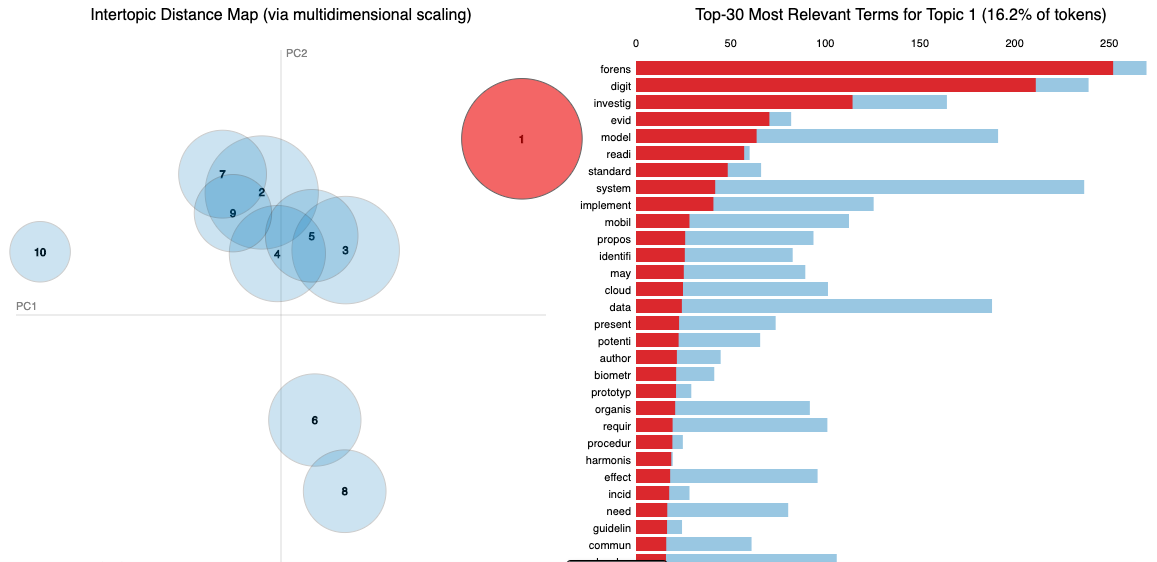
\includegraphics[width=\textwidth]{./figures/LDAVIS.png}
\caption{Visualisation package for LDA}
\label{fig:LDAVIS}
\end{figure}

Based on the coherence score and supported by the observations made in pyLDAvis, the researcher selected the LDA parameter number of topics as 20. In the next sub-section, the researcher will discuss how the similarity was calculated between the documents.

\section{Similarity between documents}

One of the main goals of this study is to present similar papers to the readers. In order to do this, the data needs to be tokenised, normalised and cleaned. After the pre-processing pipeline, the tokenised data should be transformed into a vector and fed into the latent dirichlet allocation topic modeling algorithm. After a few iterations and fine tuning of the parameters within the LDA algorithm, the output data can then be used to obtain deeper findings.

The goal of obtaining in-depth information rests on the Jensen-Shannon Divergence algorithm. As seen in Figure \ref{lst:jensenfunction}, we were computing the Jenson-Shannon Distance (JSD) using Scipy’s entropy. JSD finds the distance between an input query (LDA topic distribution of a single document) and a big matrix (the whole corpus), as seen in line 2. In line 5 it returns an array of length m, where m is the number of document in the corpus.

Later in line 5, the square root of the Jensen-Shannon Divergence is returned because the square root of Jensen-Shannon Divergence is the Jensen-Shannon Distance. The smaller the JSD, the more similar the two topic distributions are to each other; in this case, the more similar two documents are to each other.

\begin{lstlisting}[language=Python, label={lst:jensenfunction}, caption=Implementation of Jensen-Shannon similarity]
def jensen_shannon(query, matrix):
    p = query[None,:].T
    q = matrix.T
    m = 0.5*(p + q)
    return np.sqrt(0.5*(entropy(p,m) + entropy(q,m)))
\end{lstlisting}

The Jensen-Shannon function in Listing \ref{lst:jensenfunction} is then implemented in Listing \ref{lst:jensen}, where it actually computes the JSD and returns the top k smallest distances. These Jensen-Shannon distances were then used to find the recommendations of academic papers.

\begin{lstlisting}[language=Python, label={lst:jensen}, caption=Jensen-Shannon function]
def get_most_similar_documents(query,matrix,k=10):
    sims = jensen_shannon(query,matrix) 
    return sims.argsort()[:k]
\end{lstlisting}

\begin{table}[]
\begin{tabular}{|l|l|}
\hline
\textbf{Title of test paper} & \textbf{Tokenised paper} \\ \hline
\begin{tabular}[c]{@{}l@{}}Testing the harmonised digital forensic\\ investigation process model using an \\ android mobile phone\end{tabular} & \begin{tabular}[c]{@{}l@{}}{[}'test', 'harmonis', 'digit', \\ 'forens', 'investig', 'model',\\  'android', 'mobil', 'phone'{]}\end{tabular} \\ \hline
\end{tabular}
\caption{Test paper and tokenized output}
\label{tab:testdigital}
\end{table}

As mentioned in Chapter \ref{chap: Chapter 3}, the dataset was split into a training set and a testing set. The testing set comprised only one document. The document was kept aside while training the model. The test document was selected at random using a simple Python random function. The title of the test paper can be seen in Table \ref{tab:testdigital}, alongside the tokenised words from that one document corpus. Interpreting the tokenised data, a fairly good guess can be made of the content of the paper. The researcher translated the tokenised data as testing a model in the digital forensic field, looking at mobile phones, Android more specifically.

\begin{table}[]
\begin{tabular}{|l|c|}
\hline
\textbf{Title of papers} & \textbf{Scores} \\ \hline
The design of a wireless forensic readiness model (WFRM) & 0.426 \\ \hline
\begin{tabular}[c]{@{}l@{}}Mobile forensics using the harmonised digital forensic \\ Investigation process\end{tabular} & 0.452 \\ \hline
\begin{tabular}[c]{@{}l@{}}Enhancing digital business ecosystem trust and reputation with\\  centrality measures\end{tabular} & 0.498 \\ \hline
\begin{tabular}[c]{@{}l@{}}Mobile cyber-bullying: A proposal for a pre-emptive approach to risk\\  mitigation by employing digital forensic readiness\end{tabular} & 0.497 \\ \hline
Remote fingerprinting and multisensor data fusion & 0.508 \\ \hline
\begin{tabular}[c]{@{}l@{}}Real-time distributed malicious traffic monitoring for\\  Honeypots and network telescopes.\end{tabular} & 0.509 \\ \hline
Harmonised digital forensic investigation process model & 0.549 \\ \hline
Digital forensic readiness in the cloud & 0.579 \\ \hline
\begin{tabular}[c]{@{}l@{}}Towards a digital forensic readiness framework for \\ Public key infrastructure systems\end{tabular} & 0.592 \\ \hline
Bimodal biometrics for financial infrastructure security & 0.603 \\ \hline
\end{tabular}
\caption{Similarity scores of the most similar academic papers}
\label{tab:digital}
\end{table}

Looking at the JSD output of the two topic distributions, whole corpus and the one document, a recommendation can be made. In Listing \ref{tab:digital} we can see that the scores are sorted in ascending order, ranging from 0,426 to 0,603. The smaller the score, the more similar that specific document is to the test document. However, no hard-coded threshold would have made a difference in identifying the top most similar documents. These most similar documents were, in fact, closely similar to the test document.

\section{Summary}
This chapter discussed the prototype development. It outlined the importance of having a good pre-processing pipeline in place. This entailed feeding the data that was extracted from PDFs into a JSON format file and stored on Github for easy access ability. After the data was tokenised and pre-processed, it was transformed into a vector so the LDA algorithm could use the data. Through the iterations of fine tuning the parameters of the LDA model, the number of topics were chosen (20 topics) and fed into the Jensen-Shannon Divergence similarity model and the papers were all ranked, based on similarity scores. Smaller similarity scores indicates that a particular paper is very similar to the test paper. The next chapter discusses the lessons learned while developing the prototype.